\chapter{Delimitation}
In the project some limits has to be set for the use of models and materials. The objective of the control system is to prove the feasibility of using a electronic stabilization system in rockets, which has a relation to the control of the inverted pendulum. The system is developed as a proof-of-concept solution with the possibility to be adaptable for a full-scale rocket. The models in the project can only be approximations of reality, and it is therefore observable that the transfer to a full-scale rocket will not be linear though.        

\textbf{Physical delimitation:}
The inverted pendulum setup used in the projects, is pre-fabricated and made available by the university. The choice of motor, gears, and other components will therefore not be changed. The model is shown cf. figure \ref{fig:InvertedPendulum1}.

\begin{figure} [htbp]
	\centering
	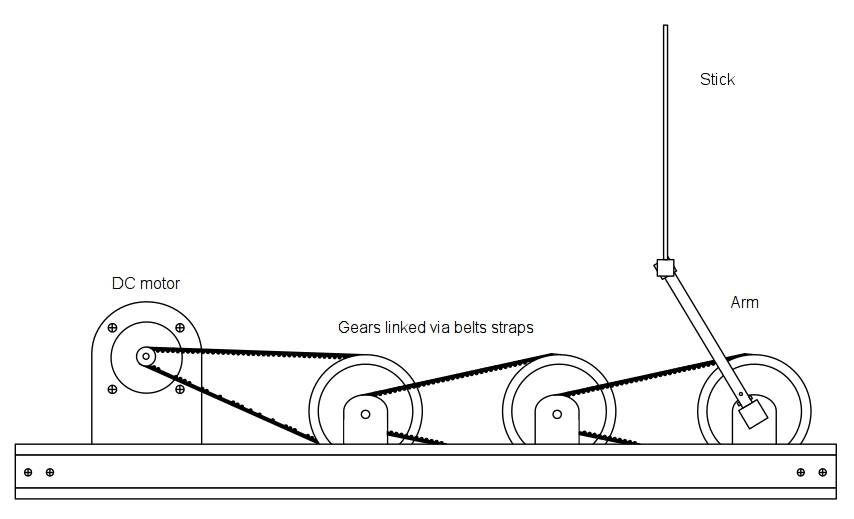
\includegraphics[width=0.8\linewidth]{figures/"Preanalysis&Requirement"/invertedPendulumDiagram}
	\caption{Diagram of the inverse pendulum setup.} \label{fig:InvertedPendulum1}
\end{figure}
\todo{Figure should be updated with lengths and gear teeth}
	
The physical parameters of the setup is seen cf. section \todo{Add reference to section Inverted Pendulum Description}

\textbf{Testing:}
TBD

\textbf{TBD:}
TBD